\chapter{Frameworks and IOC}
\section{Frameworks}

A \textbf{Software Framework}
is a collection of common code
providing generic functionality that can be selectively
overridden or specialized by user code providing
specific functionality.\\
An \textbf{Application Framework} is a software framework used to
implement the standard structure of an \textit{application} for
a specific development environment.

\labelitemize{Examples}{

   \begin{enumerate}
      \item General Software Frameworks
      \begin{enumerate}
         \item \texttt{.NET}
         \item \texttt{Android SDK}
         \item \texttt{Cocoa}
         \item \texttt{Eclipse}
      \end{enumerate}
      \item GUI Frameworks
      \begin{enumerate}
         \item \texttt{MFC}
         \item \texttt{Gnome}
         \item \texttt{Qt}
      \end{enumerate}
      \item Web Frameworks
      \begin{enumerate}
         \item \texttt{ASP.NET}
         \item \texttt{Rails}
         \item \texttt{GWT}
         \item \texttt{Spring}
         \item \texttt{Flask}
      \end{enumerate}
   \end{enumerate}
}

A framework embodies some \textit{abstract design}, with
more behavior built in.
In order to use it you need to insert your behavior into various places in the framework either by subclassing or by plugging in your own classes,
then 
the framework’s code, which handles the program's \textbf{control flow} (the "\texttt{main} execution"), then calls your code at these points.\\
This realizes a very general concept, emphasizing \textbf{inversion of
control} as opposed to libraries,
where the user's code calls the library one,
here is the code of the framework that calls the user's one.

\subsection{Component Frameworks}
\textbf{Componenent Frameworks} support development, deployment, composition
and execution of components designed according to a given
\textbf{Component Model}.
More specifically, they support \textbf{composition/connection} of components according to
the mechanisms provided by the \textit{Component Model},
allowing instances to be "plugged" into the
component framework itself,
and regulating their \textbf{interaction}.

\subsubsection{IDE and Frameworks}
\textbf{NetBeans} is both an \texttt{IDE} and supports the \texttt{JavaBeans} \textit{Component Framework}.\\
In general a framework can be supported by several \texttt{IDE}s
\note{
   e.g. \texttt{Spring} supported by \texttt{Spring Tool Suite} (based
   on \texttt{Eclipse}), \texttt{NetBeans}, \texttt{IntelliJ IDEA}, \texttt{Eclipse}, ...
} 
While an \texttt{IDE} can support several frameworks
\note{
   e.g \texttt{NetBeans} supports \texttt{JavaBeans}, \texttt{Spring}, \texttt{J2EE},
   \texttt{Maven}, \texttt{Hibernate}, \texttt{JavaServer Faces}, \texttt{Struts}, \texttt{Qt}, ...
} 

\subsection{Features}
Consist of \textbf{parts} that are found in many apps of that type
\begin{itemize}
   \item \textbf{Libraries} with APIs (classes with methods etc.)
   \item Ready-made extensible programs ("\textbf{engines}")
   \item Sometimes also \textbf{tools} (e.g. for development, configuration,
   content)
\end{itemize}
They also provide reusable abstractions of code wrapped in a well-defined API,
however recall that,unlike in libraries,
the overall program's \textbf{flow of control} is \textit{not} dictated by the caller, but by the \textit{framework}.
\nl

Frameworks usually support extensibility,
either by extending within the framework language {---} using, subclassing, overriding, implementing interfaces, registering event handlers, ...{---} or through plug-ins defined in a specific format.
 

\section{Inversion of Control}
\subsection{GUI}
In \textit{text-based interaction}, the order of interactions
and of invocations is decided by the the code,
while in the \textit{\textbf{GUI}-based interaction}, the \textit{GUI} loop decides
when to invoke the methods (listeners), based on the
order of events.

\begin{figure}[htbp]
   \centering
   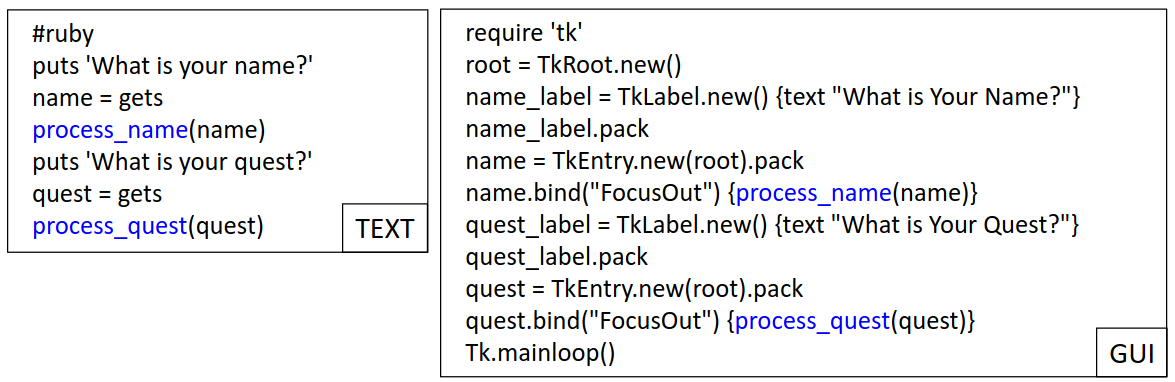
\includegraphics{images/ioc_textgui.png}
   \caption{Text vs GUI interaction}
   \label{fig:ioc_textgui}
\end{figure}

\begin{figure}[htbp]
   \centering
   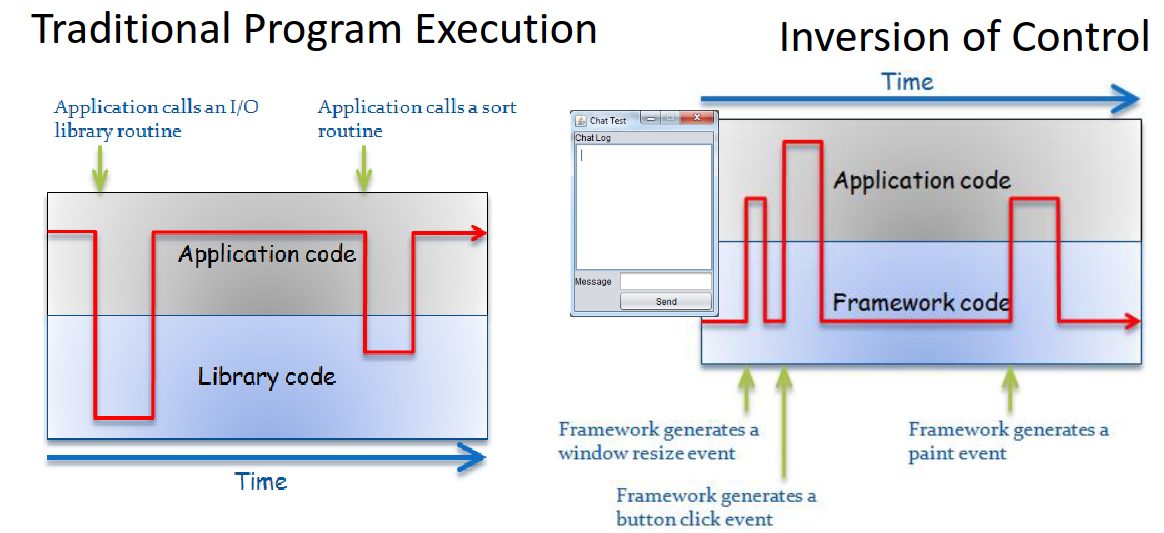
\includegraphics{images/ioc_fwvslib.png}
   \caption{IoC: Library vs Framework approach}
   \label{fig:ioc_fwvslib}
\end{figure}

\subsection{Containers}
Often Frameworks provide \textbf{containers} for deploying
\textit{components}:
a container may provide at \textit{runtime functionalities}
needed by the components to execute.

For examples \texttt{EJB} containers are responsible of the
persistent storage of data and of the availability of
\texttt{EJB}’s for all authorized clients.

\section{Loosely Coupled Systems}
Good \textit{OO Systems} should be organised as
a network of interacting objects,
keeping in mind as a goal to have \textit{high \textbf{cohesion}}, \textit{low \textbf{coupling}}.\\
Low coupling has as key advantages
\begin{itemize}
   \item Extensibility
   \item Testability
   \item Reusability
\end{itemize}

\subsection{Dependecy Injection}
When discussing \textbf{IoC} in Frameworks, \textit{"Control"} does not refer only to control flow, but also control over \textit{dependencies}, \textit{coupling}, \textit{configuration}.

We can make a few considerations on IoC with respect to dependencies:
\begin{itemize}
   \item something outside a component handles:
   \begin{itemize}
      \item configuration (properties)
      \item wiring / dependencies (components)
   \end{itemize}
   \item component-oriented
   \item removes coupling
   \begin{itemize}
      \item coupling of configuration and dependencies to the point of use
      \item coupling of component to concrete dependent components
   \end{itemize}
   \item somewhat contrary to encapsulation
\end{itemize}

\section{Trade Monitor}
Let's discuss this example to see how all of this comes into practice.
\begin{center}
   \textit{A trader wants that the system rejects trades when the exposure reaches a certain limit}
\end{center}

Thus the component (class) \texttt{TradeMonitor} provides
a method \texttt{TryTrade} (below) which checks the condition,
accessing \textit{current exposure} and \textit{exposure limit} from a \texttt{DAO} (\textit{Data Access Object}), a persistent storage.
\begin{lstlisting}
   public bool TryTrade(string symbol, int amount){
      int limit = limitDao.GetLimit(symbol);
      int exposure = limitDao.GetExposure(symbol);
      return (exposure + amount > limit) ? false : true;
      }
\end{lstlisting}
How can we limit dependencies among the two components?
\subsection{Interfaces - Refactoring 1}
Let's consider a possible refactoring, introducing \textbf{interface} and implementation separation,
which still has a static dependency on \texttt{DAO} :
\begin{figure}[htbp]
   \centering
   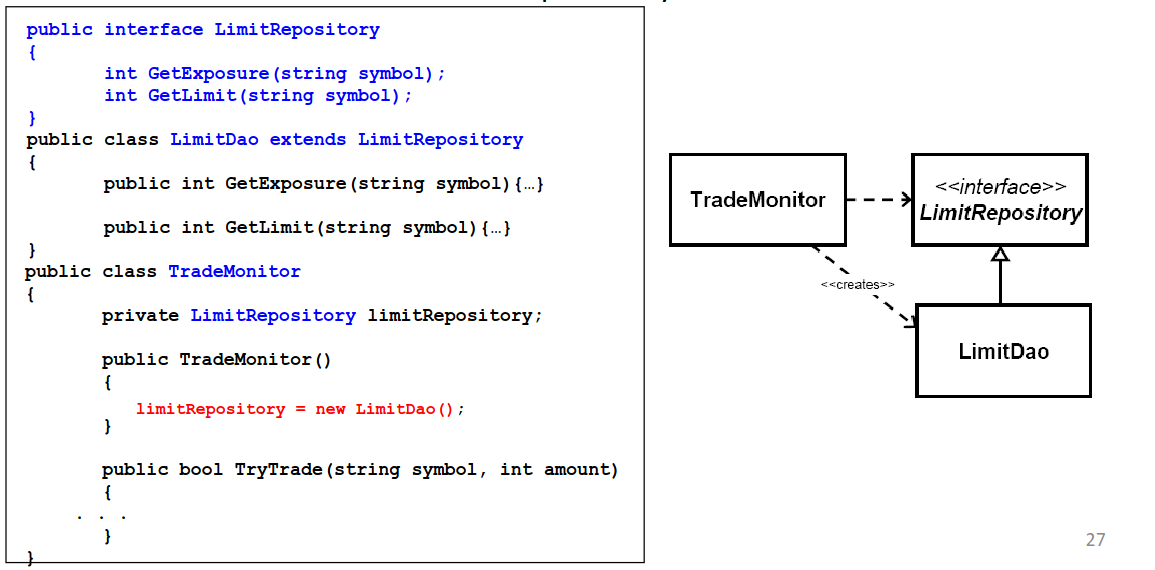
\includegraphics{images/trademonitor_ref1.png}
   \caption{Refactoring 1}
   \label{fig:trademonitor_ref1}
\end{figure}

\subsection{Factory - Refactoring 2}
Here we introduce a \textbf{factory} which resolves the previous problem, but \texttt{LimitDao} is still tightly coupled, but to \texttt{Factory}.

\begin{figure}[htbp]
   \centering
   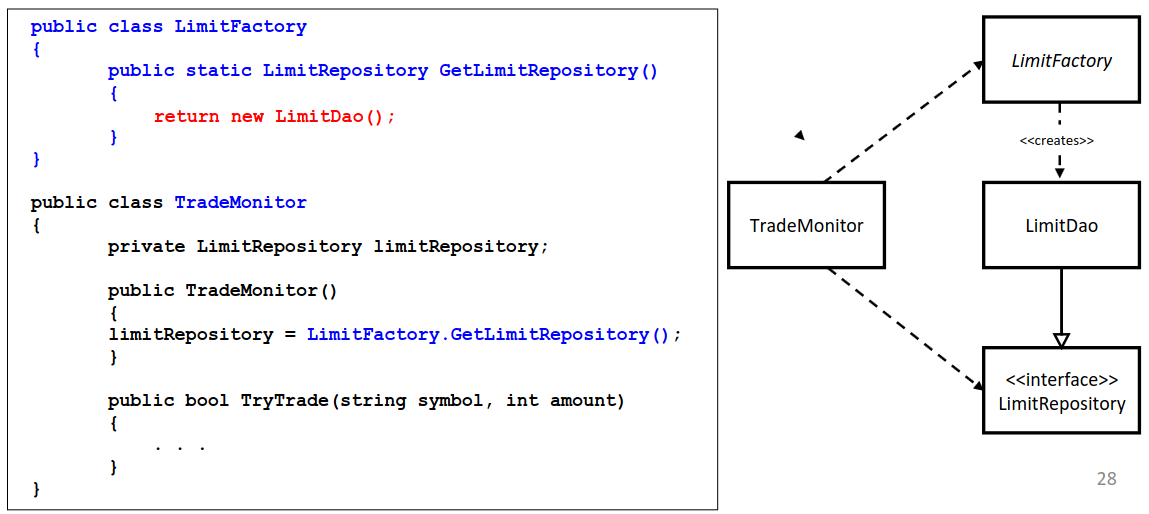
\includegraphics{images/trademonitor_ref2.png}
   \caption{Refactoring 2}
   \label{fig:trademonitor_ref2}
\end{figure}

\subsection{ServiceLocator - Refactoring 3}
Introduce a \texttt{ServiceLocator}. This object acts as a (static)
registry for the \texttt{LimitDao} you need,
giving us extensibility, testability, reusability.\\
However ote that an external \texttt{Assembler} sets up the registry.

\begin{figure}[htbp]
   \centering
   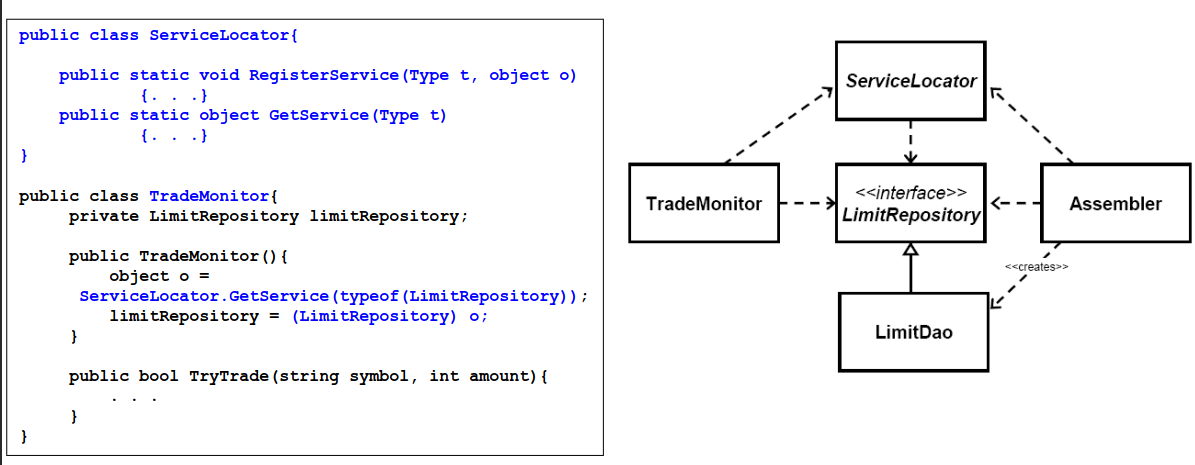
\includegraphics[width=0.7\columnwidth]{images/trademonitor_ref3.png}
   \caption{Refactoring 3}
   \label{fig:trademonitor_ref3}
\end{figure}

\labelitemize{
   \color{darkgreen}
   \textit{Pros}
}{
   \color{darkgreen}
   \begin{itemize}
      \item The Service Locator pattern succeeds in decoupling the TradeMonitor
      from the LimitDao
      \item Allows new components to be dynamically created and used by other
      components later
      \item It can be generalized in several ways, eg. to cover dynamic lookup
   \end{itemize}
}

\labelitemize{
   \color{darkred}
   \textit{Cons}
}{
   \color{darkred}
   \begin{itemize}
      \item Every component that needs a dependency must have a reference to the
      service locator
      \item All components need to be registered with the service locator
      \item If bound by name:
      \begin{itemize}
         \item Services can’t be type-checked
         \item Component has a dependency to the dependent component names
         \item if many components share an instance but later you want to specify different
      \end{itemize}
      instance for some, this becomes difficult
      \item If bound by type can only bind one instance of a type in a container
      \item Code needs to handle lookup problems
   \end{itemize}
}

\section{Dependency Injection}

\begin{figure}[htbp]
   \centering
   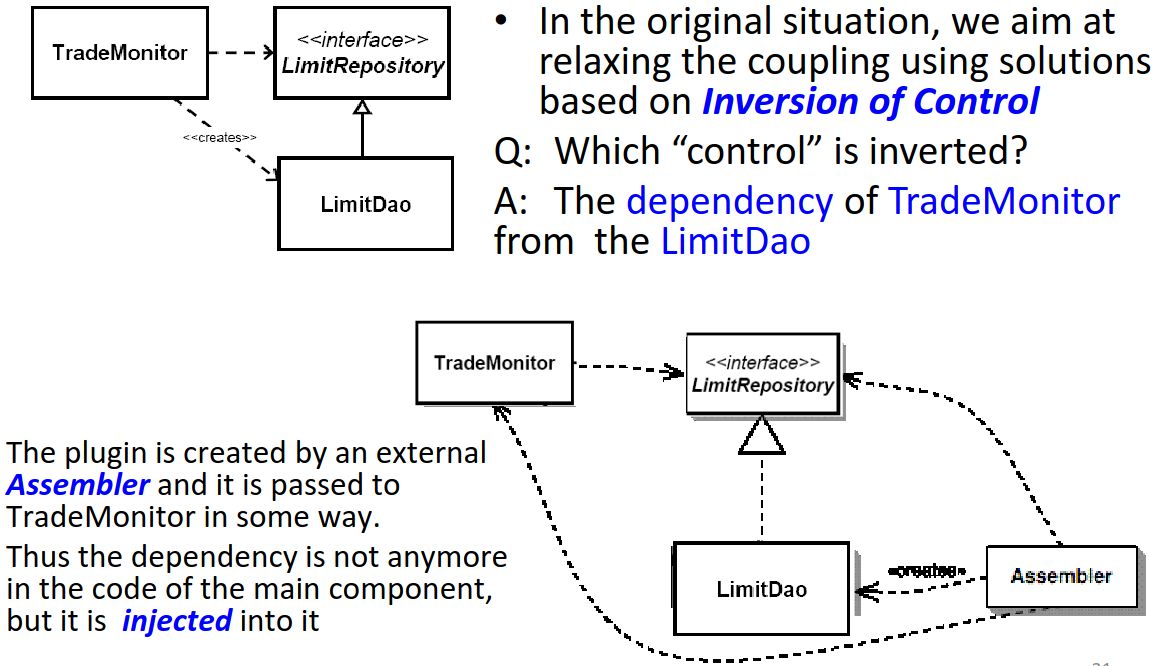
\includegraphics{images/dependency_inj.png}
   % \caption{}
   \label{fig:dependency_inj}
\end{figure}

\textbf{Dependency injection} allows avoiding \textit{hard-coded}
dependencies (strong coupling) and changing them, and allows selection among multiple implementations of a given dependency interface at run time.
It can be achieved through:
\begin{enumerate}
   \item Setter injection
   \item Constructor injection
   \item (Interface injection)
\end{enumerate}

Both \textbf{Service Locator} and \textbf{Dependency Injection} provide
the desired decoupling, but let's compare the two solutions: 
\begin{itemize}
   \item 
   With service locator there is no \textbf{IoC}, since the desired component is obtained
   after request by the \texttt{TradeMonitor} to the \texttt{Locator};
   this makes the application still depending on the locator.
   \item With dependency injection there is \textit{no explicit request}: the
   component appears in the application class.
\end{itemize}
Inversion of control is a bit harder to understand.
With Service Locator the application still depends on the
locator, besides, it is easier to find dependencies of component if \textit{Dependency Injection} is used.
% // TODO better understand service locator vs dependency injection
\begin{center}
   \color{darkgray}
   Check \textit{constructors} and \textit{setters}\\vs\\Check \textit{all invocations} to
   \texttt{Locator} in the source code
\end{center}

\section{Designing Frameworks}
Frameworks are normally implemented in an object-
oriented language such as Java.
It is important to learn to analyze a potential software family, identifying
its possible common and variable aspects, and evaluating
alternative framework architectures.
\nl

A possible idea is to start from a known divide-and-conquer algorithm such as:
\begin{lstlisting}[label={lst:divideandconquer_example},caption={Example pseudocode of a Divide-and-Conquer algorithm}]
   function solve (Problem p) returns Solution { 
      if isSimple(p)
         return simplySolve(p);
      else
         sp[] = decompose(p);
         for (i= 0; i < sp.length; i = i+1)
            sol[i] = solve(sp[i]);
         return combine(sol);
   }
\end{lstlisting}
We can apply known techniques and patterns to \textbf{define} a
\textit{framework} for a \textbf{software family}.
Instances of the defined framework, obtained by standard
extension mechanism, 
will be concrete algorithms of the \textit{family}.

\subsection{Terminology}
\begin{itemize}
   \item \textbf{Frozen Spot}\\
   common (shared) aspect of the software family
   \item \textbf{Hot Spot}\\
   variable aspect of the family
   \item \textbf{Template method}\\
   concrete method of base (abstract) class implementing behavior common to all members of the family
   \item A hot spot is represented by a group of abstract \textit{\textbf{hook} methods}.
   \item A template method calls a \textit{hook method} to invoke a function that is specific to one family member {---}Inversion of Control{---}.
   \item A hot spot is realized in a framework as hot spot subsystem:
   \begin{figure}[htbp]
      \centering
      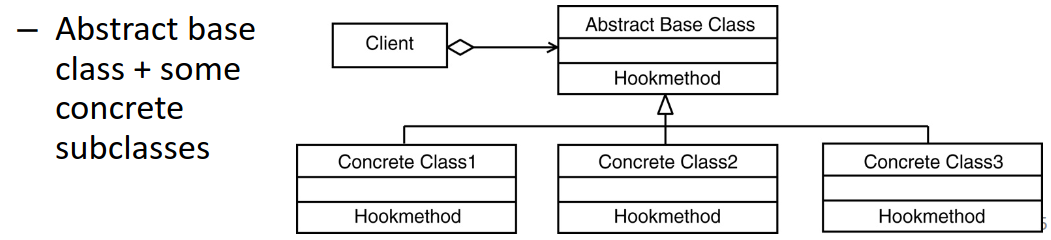
\includegraphics{images/hotspot.png}
      \caption{\textit{Hotspot} implementation}
      \label{fig:hotspot}
   \end{figure}
\end{itemize}
\labelitemize{
   \textit{Principles}
}{
   \begin{enumerate}
      \item The \textbf{unification} principle [\textit{Template Method} Design Pattern]
      \begin{enumerate}
         \item Exploits \textit{inheritance} to implement the hot spot subsystem
         \item Both the \ul{template methods and hook methods are defined in the same abstract base class}
         \item \ul{Hook methods are implemented in subclasses of the base class}
         
      \end{enumerate}
      \item The \textbf{separation} principle [\textit{Strategy} Design Pattern]
      \begin{enumerate}
         \item It uses \textit{delegation} to implement the hot spot subsystem
         \item The \ul{template methods are implemented in a \textbf{concrete} context class}; the \ul{hook methods are defined in a separate \texttt{abstract class} and implemented in its subclasses}
         \item The template methods delegate work to an instance of the
         subclass that implements the hook methods
      \end{enumerate}
   \end{enumerate}
}

\subsection{Template Method design pattern}
It is one of the behavioural pattern of the \textit{Gang of Four};
Its intent is to define the skeleton of an algorithm in an operation,
\textit{deferring} some steps to subclasses:
A \textbf{template method} belongs to an \textit{abstract} class and it defines an algorithm in terms of \textit{abstract} operations that subclasses \textbf{override}
to provide \textit{concrete behavior}.

{Template methods call, among others, the following operations:\ns
\begin{enumerate}
   \item \textbf{concrete} operations of the abstract class $\longrightarrow$ fixed parts of the algorithm
   \item \textbf{primitive} operations, $\longrightarrow$ abstract operations that subclasses have to implement
   \item \textbf{hook} operations $\longrightarrow$ provide default behavior that subclasses may override if necessary.\\
   A hook operation often does nothing by default.
\end{enumerate}}

\begin{figure}[htbp]
   \centering
   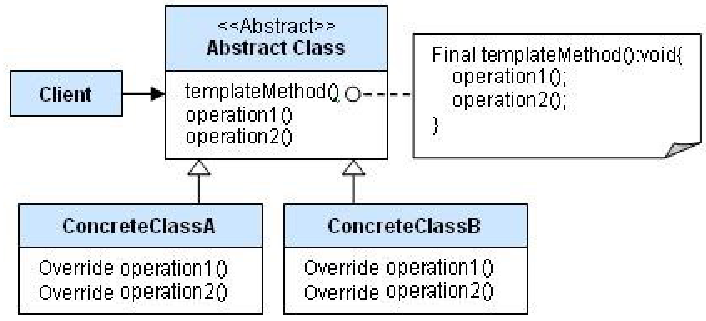
\includegraphics{images/dp_templatemethod.png}
   \caption{Template method}
   \label{fig:dp_templatemethod}
\end{figure}

\subsubsection{Applying \textit{Unification Principle}}
Let's consider the result of applying \textit{unification principle} to the example code \ref{lst:divideandconquer_example} provided before.
\lstset{
   morekeywords=[3]{solve,templatemethod},
   keywordstyle=[3]\color{green},
   morekeywords=[4]{hotspots,isSimple,simplySolve,decompose,combine},
   keywordstyle=[4]\color{red}
}
\begin{lstlisting}
   -- hotspots
   -- templatemethod
   abstract public class DivConqTemplate
   function solve (Problem p) returns Solution {
      if isSimple(p)
         return simplySolve(p);
      else
         sp[] = decompose(p);
         for (i= 0; i < sp.length; i = i+1)
            sol[i] = solve(sp[i]);
         return combine(sol);
   }
   abstract protected boolean isSimple (Problem p);
   abstract protected Solution simplySolve (Problem p);
   abstract protected Problem[] decompose (Problem p);
   abstract protected Solution combine(Problem p, Solution[] ss) ;
\end{lstlisting}
\lstset{style=javaBlock}

\begin{figure}[htbp]
   \centering
   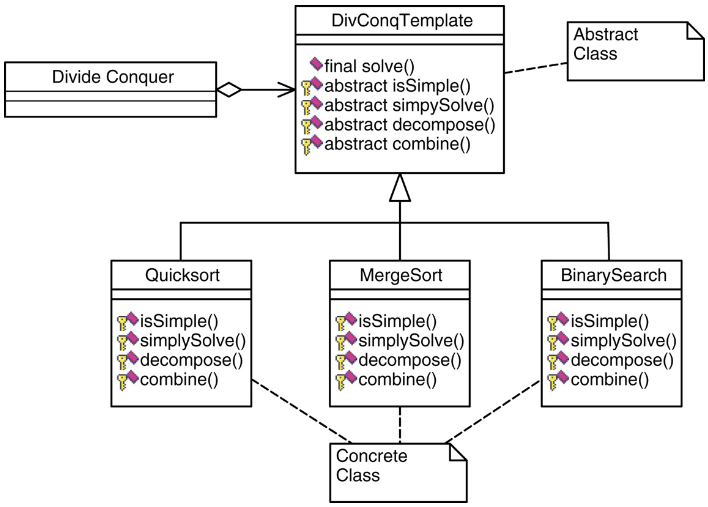
\includegraphics{images/dp_templatemethod_divide.png} 
   \caption{The generic schema of a Divide-and-Conquer \textit{Template Method} designed Framework, with the concrete implementations for various sorting algorithms.}
   \label{fig:dp_templatemethod_code}
\end{figure}

\subsection{Strategy design pattern}
Another one of the behavioural pattern of the \textit{Gang of Four};
Its intent is to allow to select (part of) an algorithm at runtime, leading the client to use an object implementing the interface and
invoking methods of the interface for the hot spots of the
algorithm.

\begin{figure}[htbp]
   \centering
   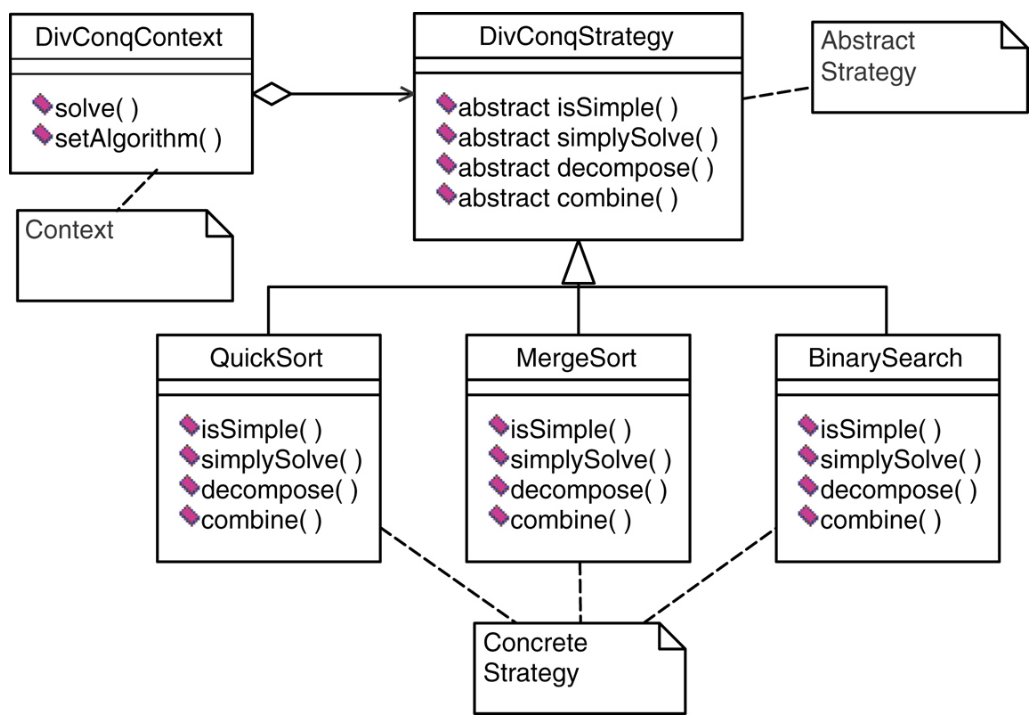
\includegraphics{images/strategyUML.png}
   \caption{Strataegy UML Class Diagram}
   \label{fig:strategyUML}
\end{figure}
\newpage
\subsubsection{Applying the \textit{Separation Principle}}
   The client delegates the hot spots to an object implementing the strategy.

   The implementations of \lstinline|DivCongStrategy| are similar to the previous case.
   
   \begin{lstlisting}
public final class DivConqContext {
   public DivConqContext(DivCongStrategy dc) {
this.dc = dc;
}

public Solution solve (Problem p)
{ Problem[] pp;
if (dc.isSimple(p)) { return dc.simplySolve(p); }
else { pp = dc.decompose(p); }
Solution[] ss = new Solution[pp.length];
for (int i = 0; i < pp.length; i++)
{  ss[i] = solve(pp[i]); }
return dc.combine(p, ss);
}

public void setAlgorithm(DivCongStrategy dc) {
   this.dc = dc;
   }
   
   private DivCongStrategy dc;
   }
\end{lstlisting}

\begin{figure}[htbp]
   \centering
   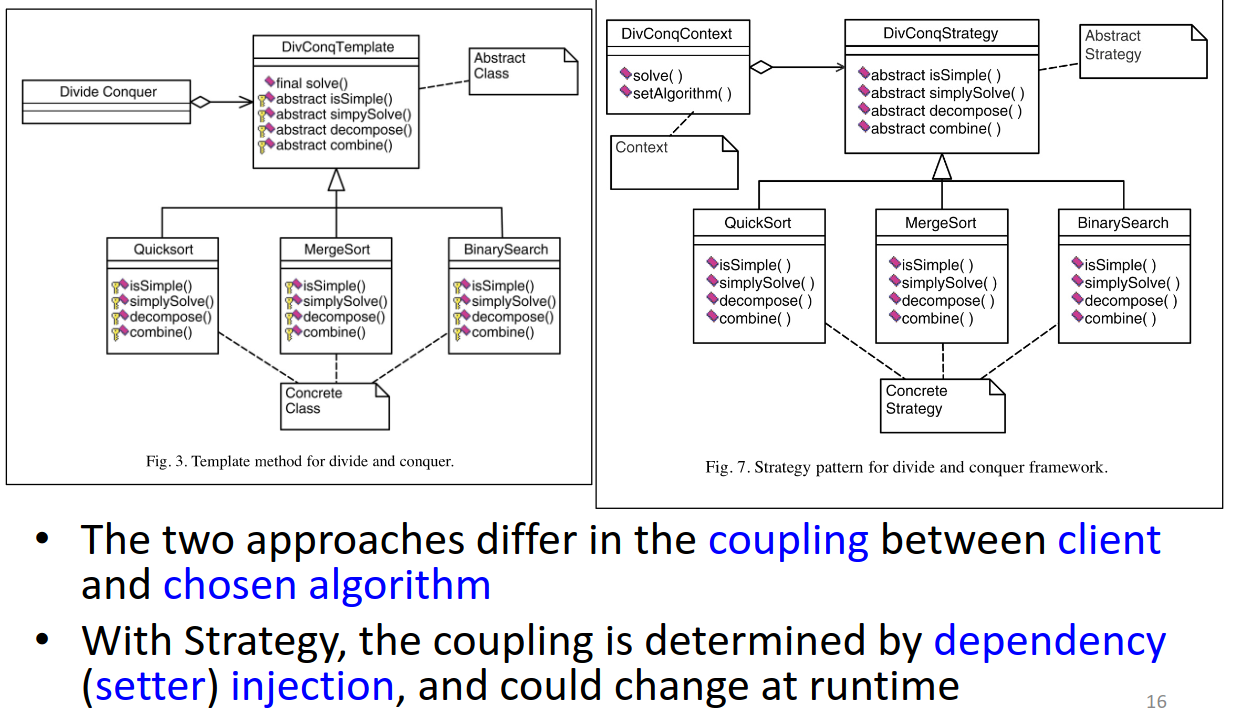
\includegraphics{images/dp_comparison.png}
   \caption{Comparison between the two pattern's schemas}
   \label{fig:dp_comparison}
\end{figure}

\section{Development by generalization}

Recalling what said earlier, we try to address:
\begin{center}
   \textit{Learning to analyze a potential software \textbf{family}, identifying its
   possible common and variable aspects, and evaluating
   alternative framework architectures. Framework design involves
   incrementally \textbf{evolving} a design rather than discovering it in one
   single step}
\end{center}

Where the \emph{evolution} consists of examining \textbf{existing designs} for family members, identifying the \textbf{frozen} and \textbf{hot spots} of the family, and ultimately \textbf{generalizing} the program structure to enable \textit{code reusing} for frozen spots and
multiple \textit{different implementations} for each hot spot.

\ul{In the slides} there is an example based on binary tree traversals, with a discussion on each generalization step.

\begin{figure}[htbp]
   \centering
   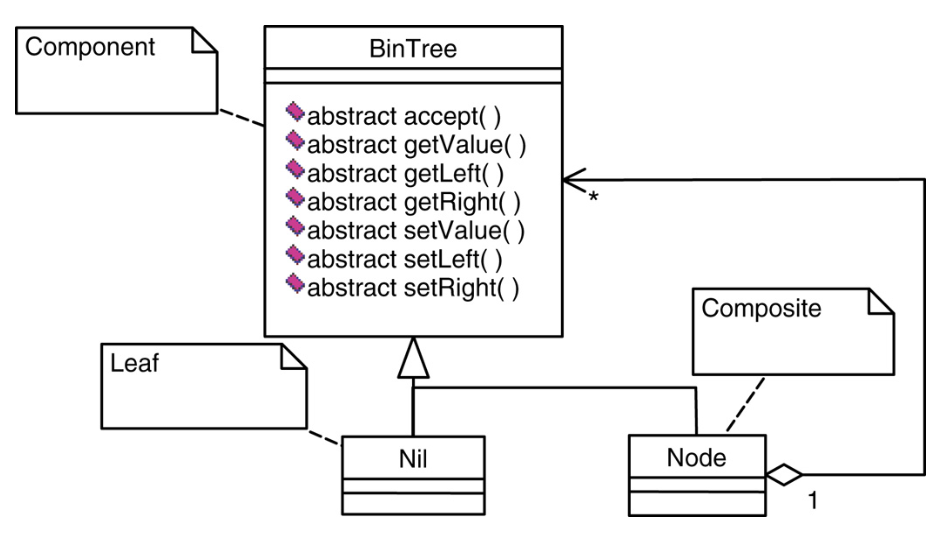
\includegraphics{images/bintree_composite.png}
   \caption{Binary tree using the Composite design pattern}
   \label{fig:}
\end{figure}

\subsection{Identifying Frozen and Hot spots}
\textbf{Frozen Spots}, which are fixed for the whole family:
\begin{enumerate}
   \item The structure of the tree, as defined by the
   BinTree hierarchy
   \item A traversal accesses every element of the tree
   once, but it can stop before completing
   \item A traversal performs one or more visit actions
   accessing an element of the tree
   \note{
      meaning that there may be different and multiple actions after visiting a node,
      since it may represent the end of a left subtree visit, a right subtree visit or a root.}
\end{enumerate}

Let's identify possible \textbf{Hot Spots}, which have to be fixed in each element of the family.
\begin{enumerate}
   \item Variability in the visit operation’s \textbf{action}:
   a function of the current node’s value and the accumulated result
   \item Variability in \textbf{ordering} of the visit \textit{action} with respect to subtree traversals;
   Should support \textit{preorder},
   \textit{postorder}, \textit{in-order}, and their combination.
   \item Variability in the \textbf{tree navigation} technique. 
   Should support any access order.
   \note{not only left-to-right, depth-first, total traversals}
\end{enumerate}

\newpage
\section{Visitor Pattern}
\begin{paracol}{2}
   \colfill
   The \textbf{Visitor} pattern guarantees \textit{separation} between algorithm
   and data structure.
   \nl

   The data structure can be made of different types of components (\textit{ConcreteElements}), and each component implements an
   \lstinline|accept(Visitor)| method.
   The \lstinline|Visitor| defines one visit method
   for each type, including the navigation logic in itself.
   At each step, the correct visit method
   is selected by \textbf{overloading}.
   \colfill
   \switchcolumn

   \begin{figure}[htbp]
      \centering
      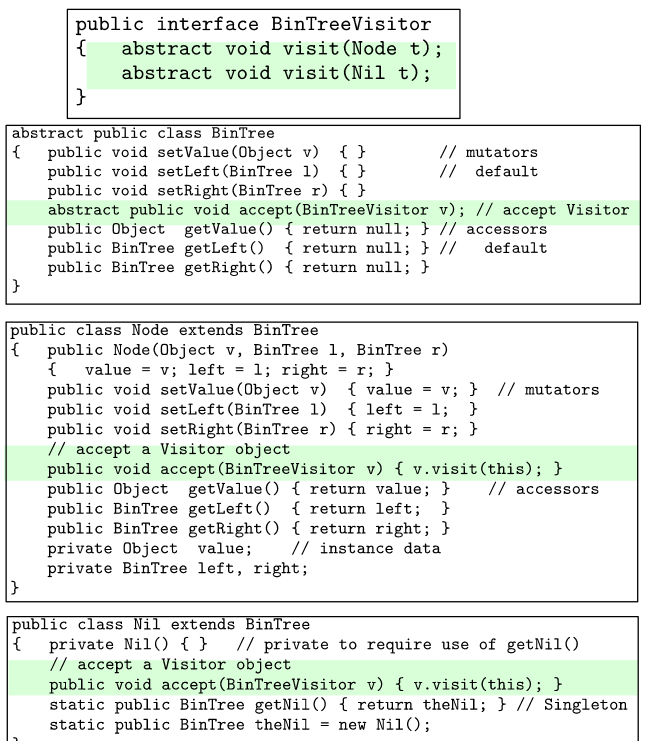
\includegraphics[width=0.9\columnwidth]{images/visitorpattern_treecode.png}
      \caption{Visitor Pattern applied to the BinTree visit}
      \label{fig:visitorpattern_treecode}
   \end{figure}
\end{paracol}

Even if in the \textit{Visitor} pattern, as in the \textit{Template Method} pattern, an abstract class is defined and later implemented by subclasses which provide concrete behaviour,
in the \textit{Visitor} pattern such classes are \textit{\textbf{intended}} to be used directly by \textit{clients},
while in the \textit{Template Method} pattern they are \textit{\textbf{intended}} to be called by the \textit{Frozen Spots} inside the abstract class itself, not by \textit{clients}.

\subsection{Wrap Up and Comparison}

The \textbf{Visitor} Pattern
consists of "Visitees" or "Hosts" and "Visitors". Hosts are objects within an object tree, and Visitors contain operations to be performed on these Hosts.

Hosts expose an \texttt{Accept()} method, which takes a Visitor object, and Visitors expose a \texttt{Visit()} method which has an overload for each Host. When the \texttt{Accept()} method is called on the Host, and a Visitor passed, a \texttt{Visit()} method is called on the visitor.

Using this pattern, \ul{operations} become \textit{Double Dispatch},\ul{ meaning they are executed based on two classes: the Host and the Visitor}.
\nl

The \textbf{Strategy} Pattern consists of a ``Context'' and a ``Strategy''. Contexts are \st{objects within a tree} related classes, and a Strategy is a class containing a series of operations to be used by the Contexts.

Strategy provides an interface of which Context objects are aware. When a Context object is created, a Strategy is also created (if not static) and given to the Context. Operations can then be selected from the selected Strategy as desired.